\begin{frame}{layering violation}
    \begin{itemize}
    \item previously router only handled IP (network layer)
    \item but looking at UDP/TCP fields
    \vspace{.5cm}
    \item router typically doesn't do defragmentation
    \item might interpret TCP/UDP fields different than end-host
    \end{itemize}
\end{frame}

\begin{frame}[fragile]{fragmented SYN}
    \begin{itemize}
    \item \verb|tcp flags & (fin|syn|rst|ack) == syn drop|
    \end{itemize}
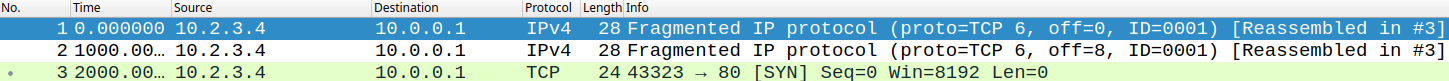
\includegraphics[width=\textwidth]{../fire/tcp-syn-frag}
    \begin{itemize}
    \item tcp flags are not first fragment
    \item need to reassemble to accurately filter
    \item \ldots or maybe filter out very short fragments
    \end{itemize}
\end{frame}

\begin{frame}[fragile]{ambiguous fragmentation}
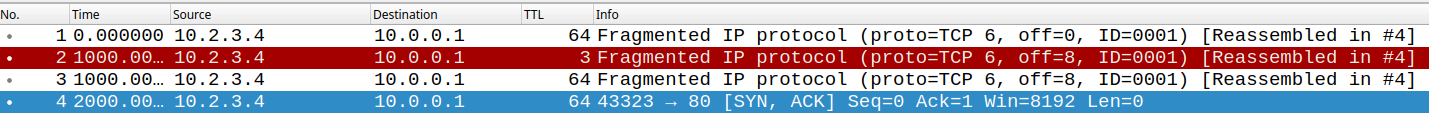
\includegraphics[width=\textwidth]{../fire/tcp-syn-ambig-frag}
    \begin{itemize}
    \item can have two different versions of a fragment
    \item using different TTLs to choose which one makes it
    \vspace{.5cm}
    \item one idea: defragment to choose which version 
        \begin{itemize}
        \item and drop unknown fragments
        \end{itemize}
    \end{itemize}
\end{frame}

\begin{frame}[fragile]{other interpretation issues}
\begin{itemize}
\item wrote: \verb+tcp flags & (fin|syn|rst|ack) == syn drop+
\item versus:\verb+tcp flags == syn drop+
\item ``mishandles'':
    \begin{itemize}
    \item SYN | ECE ?
    \item SYN | URG 
    \item SYN | first reserved flag bit?
    \item \ldots
    \end{itemize}
\item some of these combinations not defined by TCP standard
    \begin{itemize}
    \item don't really know if they open connection
    \item don't really know if they might be used for other purpose
    \end{itemize}
\item probably related to why ECN often filtered
\end{itemize}
\end{frame}

\begin{frame}[fragile]{higher-level filtering?}
    \begin{itemize}
    \item let's say we want to disallow
    \item \verb|GET /malicious HTTP/1.1|, etc.
    \vspace{.5cm}
    \item one idea: check for \verb|GET /malicious|
    \item huge number of issues:
        \begin{itemize}
        \item what if split across multiple TCP packets?
        \item what if uploading file containing \verb|GET /malicious|?
        \item what about \verb|GET   /malicious|, \verb|GET /%6dalicious|?
        \item \ldots
        \end{itemize}
    \end{itemize}
\end{frame}
